\chapter{Технологическая часть}

В этом разделе рассматривается процесс выбора инструментов для реализации базы данных и приложения. Описывается создание сущностей, заданных ограничений целостности и пользовательских ролей в разработанной базе данных. Также приведена реализация хранимой процедуры и результаты её тестирования. Дополнительно представлен интерфейс разработанного программного обеспечения.


\section{Выбор СУБД}

Наиболее распространенными CУБД реляционной модели БД являются:

\begin{itemize}[label=---]
    \item PostgreSQL~\cite{psql};
    \item SQLite~\cite{sqlite};
    \item MySQL~\cite{mysql};
    \item MSSQL~\cite{mssql}.
\end{itemize}

Для сравнения СУБД были выделены следующие критерии:
\begin{itemize}[label=---]
    \item возможность создания ролевой модели;
    \item соответствие всем SQL стандартам ANSI/ISO~\cite{ansi_iso};
    \item наличие Row-Level Security (RLS).
\end{itemize}

В таблице~\ref{table:rel_sql_comp} представлены результаты сравнения наиболее распространенных реляционных СУБД по выбранным критериям.

\begin{table}[H]
    \begin{center}
        \caption{Сравнение распространенных реляционных СУБД}
        \begin{tabular}{|c|c|c|c|c|}
            \hline
             & PostgreSQL & SQLite & MySQL & MSSQL \\
            \hline
            Создание ролей & + & -- & ± & + \\
            \hline
            \makecell{Соответствие\\ SQL стандартам} & + & -- & ± & ± \\
            \hline
            Row-Level Security & + & -- & + & + \\
            \hline
        \end{tabular}
        \label{table:rel_sql_comp}
    \end{center}
\end{table}

В рамках данной работы в качестве СУБД была выбрана PostgreSQL, так как она обладает достаточным функционалом для поставленной цели.

\section{Средства реализации}

Для реализации программного обеспечения выбран язык $Rust$~\cite{rust-book}. Выбор был сделан на основании того, что данный язык поддерживает все типы данных, определенные на этапе проектирования, и предоставляет полный набор возможностей, необходимых для реализации поставленной задачи. Для реализации сервера был выбран фреймворк $axum$~\cite{axum-crate}. Для реализации компонента доступа к данным был выбран фреймворк $sqlx$~\cite{sqlx-crate}.

Для реализации клиента был выбран язык $Swift$~\cite{swift-lang}, который позволяет разрабатывать приложения под $iOS$. Для реализации интерфейса был выбран фреймворк $UIKit$~\cite{uikit-fw}, который включает стандартные компоненты пользовательского интерфейса, поддерживает обработку ввода и жестов, а также обеспечивает анимации и переходы между экранами.


\section{Реализация}

\subsection{Создание таблиц}

В листингах~\ref{tablecreate-1}---\ref{tablecreate-10} приведены запросы для создания таблиц и ограничений целостности базы данных.

\begin{center}
\captionsetup{justification=raggedright,singlelinecheck=off}
\begin{lstlisting}[label=tablecreate-1, caption=Создание таблицы AppUser]
CREATE TABLE AppUser (
    id SERIAL PRIMARY KEY,
    login TEXT NOT NULL,
    password TEXT NOT NULL,
    role TEXT NOT NULL,
    name TEXT NOT NULL,
    surname TEXT NOT NULL,
    lastname TEXT,
    is_verified BOOLEAN DEFAULT FALSE,
    passport_serial INTEGER,
    passport_num INTEGER
);

ALTER TABLE AppUser
    ADD CONSTRAINT unique_passport UNIQUE (passport_serial, passport_num),
    ADD CONSTRAINT check_role CHECK (role IN ('user', 'operator', 'audit')),
    ADD CONSTRAINT unique_login UNIQUE (login),
    ADD CONSTRAINT check_login_email CHECK (login ~ '^[A-Za-z0-9._%+-]+@[A-Za-z0-9.-]+\.[A-Za-z]{2,}$'),
    ADD CONSTRAINT check_passport_format CHECK (passport_serial BETWEEN 1 AND 9999 AND passport_num BETWEEN 1 AND 999999);
\end{lstlisting}
\end{center}

\begin{center}
\captionsetup{justification=raggedright,singlelinecheck=off}
\begin{lstlisting}[label=tablecreate-2, caption=Создание таблицы Car]
CREATE TABLE Car (
    id SERIAL PRIMARY KEY,
    owner_id INTEGER NOT NULL,
    mark TEXT NOT NULL,
    model TEXT NOT NULL,
    vin TEXT NOT NULL,
    mileage INTEGER NOT NULL,
    color TEXT NOT NULL
);

ALTER TABLE Car
    ADD FOREIGN KEY (owner_id) REFERENCES CarOwner(id) ON DELETE CASCADE,
    ADD CONSTRAINT unique_vin UNIQUE (vin),
    ADD CONSTRAINT check_mileage CHECK (mileage >= 0),
    ADD CONSTRAINT check_vin_length CHECK (LENGTH(vin) = 17);
\end{lstlisting}
\end{center}

\begin{center}
\captionsetup{justification=raggedright,singlelinecheck=off}
\begin{lstlisting}[label=tablecreate-3, caption=Создание таблицы CarOwner]
CREATE TABLE CarOwner (
    id SERIAL PRIMARY KEY,
    name TEXT NOT NULL,
    surname TEXT NOT NULL,
    lastname TEXT,
    age INTEGER NOT NULL,
    drive_exp INTEGER NOT NULL,
    passport_serial INTEGER NOT NULL,
    passport_num INTEGER NOT NULL,
    drive_license_serial INTEGER NOT NULL,
    drive_license_num INTEGER NOT NULL
);

ALTER TABLE CarOwner
    ADD CONSTRAINT unique_owner_passport UNIQUE (passport_serial, passport_num),
    ADD CONSTRAINT unique_drive_license UNIQUE (drive_license_serial, drive_license_num),
    ADD CONSTRAINT check_age CHECK (age >= 18),
    ADD CONSTRAINT check_drive_exp CHECK (drive_exp >= 0),
    ADD CONSTRAINT check_owner_passport_format CHECK (passport_serial BETWEEN 1 AND 9999 AND passport_num BETWEEN 1 AND 999999),
    ADD CONSTRAINT check_drive_license_format CHECK (drive_license_serial BETWEEN 1 AND 9999 AND drive_license_num BETWEEN 1 AND 999999);
\end{lstlisting}
\end{center}

\begin{center}
\captionsetup{justification=raggedright,singlelinecheck=off}
\begin{lstlisting}[label=tablecreate-4, caption=Создание таблицы PTS]
CREATE TABLE PTS (
    id SERIAL PRIMARY KEY,
    sts_id INTEGER NOT NULL,
    pts_serial INTEGER NOT NULL,
    pts_number INTEGER NOT NULL,
    import_country TEXT NOT NULL
);

ALTER TABLE PTS
    ADD FOREIGN KEY (sts_id) REFERENCES STS(id) ON DELETE CASCADE,
    ADD CONSTRAINT unique_pts UNIQUE (pts_serial, pts_number),
    ADD CONSTRAINT check_pts_format CHECK (pts_serial BETWEEN 1 AND 9999 AND pts_number BETWEEN 1 AND 999999);
\end{lstlisting}
\end{center}

\begin{center}
\captionsetup{justification=raggedright,singlelinecheck=off}
\begin{lstlisting}[label=tablecreate-5, caption=Создание таблицы STS]
CREATE TABLE STS (
    id SERIAL PRIMARY KEY,
    car_id INTEGER NOT NULL,
    owner_id INTEGER NOT NULL,
    vin TEXT NOT NULL,
    gos_num TEXT NOT NULL,
    mark TEXT NOT NULL,
    model TEXT NOT NULL,
    horse_power INTEGER,
    car_weight INTEGER,
    sts_serial INTEGER NOT NULL,
    sts_num INTEGER NOT NULL,
    engine_type TEXT NOT NULL,
    car_class TEXT NOT NULL,
    release_date DATE NOT NULL,
    reg_date DATE NOT NULL
);
ALTER TABLE STS
    ADD FOREIGN KEY (car_id) REFERENCES Car(id) ON DELETE CASCADE,
    ADD FOREIGN KEY (owner_id) REFERENCES CarOwner(id) ON DELETE CASCADE,
    ADD CONSTRAINT unique_sts UNIQUE (sts_serial, sts_num),
    ADD CONSTRAINT unique_gos_num UNIQUE (gos_num),
    ADD CONSTRAINT sts_unique_vin UNIQUE (vin),
    ADD CONSTRAINT check_horse_power CHECK (horse_power > 0),
    ADD CONSTRAINT check_weight CHECK (car_weight > 0),
    ADD CONSTRAINT check_engine_type CHECK (engine_type IN ('petrol', 'diesel', 'electric', 'hybrid')),
    ADD CONSTRAINT check_car_class CHECK (car_class IN ('A', 'B', 'C', 'D', 'E', 'F', 'S', 'M', 'J')),
    ADD CONSTRAINT check_release_date CHECK (release_date <= CURRENT_DATE),
    ADD CONSTRAINT check_reg_date CHECK (reg_date >= release_date),
    ADD CONSTRAINT check_sts_format CHECK (sts_serial BETWEEN 1 AND 9999 AND sts_num BETWEEN 1 AND 999999),
    ADD CONSTRAINT check_gos_num_format CHECK (gos_num ~ '^[АВЕКМНОРСТУХ]\d{3}[АВЕКМНОРСТУХ]{2}\d{2,3}\$'),
    ADD CONSTRAINT check_vin_length CHECK (LENGTH(vin) = 17);
\end{lstlisting}
\end{center}

\begin{center}
\captionsetup{justification=raggedright,singlelinecheck=off}
\begin{lstlisting}[label=tablecreate-6, caption=Создание таблицы OwnerHistory]
CREATE TABLE OwnerHistory (
    id SERIAL PRIMARY KEY,
    pts_id INTEGER NOT NULL,
    mileage INTEGER NOT NULL,
    reg_date DATE NOT NULL,
    dereg_date DATE
);

ALTER TABLE OwnerHistory
    ADD FOREIGN KEY (pts_id) REFERENCES PTS(id) ON DELETE CASCADE,
    ADD CONSTRAINT check_mileage CHECK (mileage >= 0),
    ADD CONSTRAINT check_dates CHECK (dereg_date IS NULL OR dereg_date >= reg_date);
\end{lstlisting}
\end{center}

\begin{center}
\captionsetup{justification=raggedright,singlelinecheck=off}
\begin{lstlisting}[label=tablecreate-7, caption=Создание таблицы OwnerHistoryOwner]
CREATE TABLE OwnerHistoryOwner (
    id SERIAL PRIMARY KEY,
    owner_id INTEGER NOT NULL,
    owner_history_id INTEGER NOT NULL
);

ALTER TABLE OwnerHistoryOwner
    ADD FOREIGN KEY (owner_id) REFERENCES CarOwner(id) ON DELETE CASCADE,
    ADD FOREIGN KEY (owner_history_id) REFERENCES OwnerHistory(id) ON DELETE CASCADE;
\end{lstlisting}
\end{center}

\begin{center}
\captionsetup{justification=raggedright,singlelinecheck=off}
\begin{lstlisting}[label=tablecreate-8, caption=Создание таблицы Camera]
CREATE TABLE Camera (
    id SERIAL PRIMARY KEY,
    longitude DOUBLE PRECISION NOT NULL,
    latitude DOUBLE PRECISION NOT NULL,
    install_date DATE NOT NULL,
    is_radar BOOLEAN DEFAULT FALSE
);

ALTER TABLE Camera
    ADD CONSTRAINT check_install_date CHECK (install_date <= CURRENT_DATE);
\end{lstlisting}
\end{center}

\begin{center}
\captionsetup{justification=raggedright,singlelinecheck=off}
\begin{lstlisting}[label=tablecreate-9, caption=Создание таблицы CarSnapshot]
CREATE TABLE CarSnapshot (
    id SERIAL PRIMARY KEY,
    camera_id INTEGER NOT NULL,
    snap_datetime TIMESTAMP NOT NULL,
    speed INTEGER,
    gos_num TEXT NOT NULL,
    road_line INTEGER
);

ALTER TABLE CarSnapshot
    ADD FOREIGN KEY (camera_id) REFERENCES Camera(id) ON DELETE CASCADE,
    ADD CONSTRAINT check_speed CHECK (speed >= 0),
    ADD CONSTRAINT check_road_line CHECK (road_line >= 0),
    ADD CONSTRAINT check_gos_num_format CHECK (gos_num ~ '^[АВЕКМНОРСТУХ]\d{3}[АВЕКМНОРСТУХ]{2}\d{2,3}$'),
    ADD CONSTRAINT check_snapshot_date CHECK (snap_datetime <= (NOW() AT TIME ZONE 'Europe/Moscow' + INTERVAL '5 seconds'));
\end{lstlisting}
\end{center}

\begin{center}
\captionsetup{justification=raggedright,singlelinecheck=off}
\begin{lstlisting}[label=tablecreate-10, caption=Создание таблицы TrackInfo]
CREATE TABLE TrackInfo (
    id SERIAL PRIMARY KEY,
    user_id INTEGER NOT NULL,
    track_time TIMESTAMP NOT NULL,
    route_date DATE NOT NULL,
    car_id INTEGER NOT NULL
);

ALTER TABLE TrackInfo
    ADD FOREIGN KEY (user_id) REFERENCES AppUser(id) ON DELETE CASCADE,
    ADD FOREIGN KEY (car_id) REFERENCES Car(id) ON DELETE CASCADE,
    ADD CONSTRAINT check_route_date CHECK (route_date <= track_time::DATE);
\end{lstlisting}
\end{center}

\subsection{Создание ролей}

В листингах~\ref{roles-1}---~\ref{roles-4}  представлено создание ролей базы данных.

\begin{center}
\captionsetup{justification=raggedright,singlelinecheck=off}
\begin{lstlisting}[label=roles-1, caption=Активация Row-Level Security (RLS)]
ALTER TABLE Car ENABLE ROW LEVEL SECURITY;
ALTER TABLE CarOwner ENABLE ROW LEVEL SECURITY;
ALTER TABLE STS ENABLE ROW LEVEL SECURITY;
ALTER TABLE PTS ENABLE ROW LEVEL SECURITY;
ALTER TABLE OwnerHistory ENABLE ROW LEVEL SECURITY;
ALTER TABLE OwnerHistoryOwner ENABLE ROW LEVEL SECURITY;
\end{lstlisting}
\end{center}

\begin{center}
\captionsetup{justification=raggedright,singlelinecheck=off}
\begin{lstlisting}[label=roles-2, caption=Создание роли оператора]
CREATE ROLE operator_role WITH
    NOSUPERUSER
    NOCREATEDB
    NOCREATEROLE
    NOINHERIT
    NOREPLICATION
    NOBYPASSRLS
    CONNECTION LIMIT -1
    LOGIN
    PASSWORD 'Oper@tor123';

GRANT SELECT ON 
    AppUser,
    Car,
    CarSnapshot,
    Camera,
    CarOwner,
    PTS,
    OwnerHistory,
    OwnerHistoryOwner,
    STS
TO operator_role;

CREATE POLICY operator_car_access ON Car
FOR SELECT TO operator_role
USING (true);

CREATE POLICY operator_carowner_access ON CarOwner
FOR SELECT TO operator_role
USING (true);

CREATE POLICY operator_sts_access ON STS
FOR SELECT TO operator_role
USING (true);

CREATE POLICY operator_pts_access ON PTS
FOR SELECT TO operator_role
USING (true);

CREATE POLICY operator_ownerhistory_access ON OwnerHistory
FOR SELECT TO operator_role
USING (true);

CREATE POLICY operator_ownerhistoryowner_access ON OwnerHistoryOwner
FOR SELECT TO operator_role
USING (true);
\end{lstlisting}
\end{center}

\begin{center}
\captionsetup{justification=raggedright,singlelinecheck=off}
\begin{lstlisting}[label=roles-3, caption=Создание роли аудита]
CREATE ROLE audit_role WITH
    NOSUPERUSER
    NOCREATEDB
    NOCREATEROLE
    NOINHERIT
    NOREPLICATION
    NOBYPASSRLS
    CONNECTION LIMIT -1
    LOGIN
    PASSWORD 'Aud1t$ecure';

GRANT SELECT ON 
    AppUser,
    Car,
    TrackInfo,
    CarOwner,
    PTS,
    OwnerHistory,
    OwnerHistoryOwner,
    STS
TO audit_role;

CREATE POLICY audit_car_access ON Car
FOR SELECT TO audit_role
USING (true);

CREATE POLICY audit_carowner_access ON CarOwner
FOR SELECT TO audit_role
USING (true);

CREATE POLICY audit_sts_access ON STS
FOR SELECT TO audit_role
USING (true);

CREATE POLICY audit_pts_access ON PTS
FOR SELECT TO audit_role
USING (true);

CREATE POLICY audit_ownerhistory_access ON OwnerHistory
FOR SELECT TO audit_role
USING (true);

CREATE POLICY audit_ownerhistoryowner_access ON OwnerHistoryOwner
FOR SELECT TO audit_role
USING (true);
\end{lstlisting}
\end{center}

\begin{center}
\captionsetup{justification=raggedright,singlelinecheck=off}
\begin{lstlisting}[label=roles-4, caption=Создание роли пользователя]
CREATE ROLE user_role WITH
    NOSUPERUSER
    NOCREATEDB
    NOCREATEROLE
    NOINHERIT
    NOREPLICATION
    NOBYPASSRLS
    CONNECTION LIMIT -1
    LOGIN
    PASSWORD 'Us3rP@ssword';

GRANT SELECT ON 
    Car,
    PTS,
    OwnerHistory,
    OwnerHistoryOwner,
    STS,
    CarOwner
TO user_role;

CREATE POLICY user_carowner_access ON CarOwner
FOR SELECT TO user_role
USING (
    passport_serial = current_setting('app.passport_serial')::INTEGER AND
    passport_num = current_setting('app.passport_num')::INTEGER
);

CREATE POLICY user_car_access ON Car
FOR SELECT TO user_role
USING (
    id IN (
        SELECT car_id FROM CarOwner
        WHERE passport_serial = current_setting('app.passport_serial')::INTEGER
          AND passport_num = current_setting('app.passport_num')::INTEGER
    )
);

CREATE POLICY user_sts_access ON STS
FOR SELECT TO user_role
USING (
    car_id IN (
        SELECT id FROM Car
        WHERE id IN (
            SELECT car_id FROM CarOwner
            WHERE passport_serial = current_setting('app.passport_serial')::INTEGER
              AND passport_num = current_setting('app.passport_num')::INTEGER
        )
    )
);

CREATE POLICY user_pts_access ON PTS
FOR SELECT TO user_role
USING (
    sts_id IN (
        SELECT id FROM STS
        WHERE car_id IN (
            SELECT car_id FROM CarOwner
            WHERE passport_serial = current_setting('app.passport_serial')::INTEGER
              AND passport_num = current_setting('app.passport_num')::INTEGER
        )
    )
);

CREATE POLICY user_ownerhistory_access ON OwnerHistory
FOR SELECT TO user_role
USING (
    pts_id IN (
        SELECT id FROM PTS
        WHERE sts_id IN (
            SELECT id FROM STS
            WHERE car_id IN (
                SELECT car_id FROM CarOwner
                WHERE passport_serial = current_setting('app.passport_serial')::INTEGER
                  AND passport_num = current_setting('app.passport_num')::INTEGER
            )
        )
    )
);

CREATE POLICY user_ownerhistoryowner_access ON OwnerHistoryOwner
FOR SELECT TO user_role
USING (
    owner_id IN (
        SELECT id FROM CarOwner
        WHERE passport_serial = current_setting('app.passport_serial')::INTEGER
          AND passport_num = current_setting('app.passport_num')::INTEGER
    )
);
\end{lstlisting}
\end{center}

\subsection{Создание и тестирование процедуры}

Реализация процедуры обновления паспортных данных представлена в листинге~\ref{lst:proc}. На вход функции подаются логин пользователя и новые паспортные данные(серия и номер). В случае успеха функция обновит пасспортные данные пользователя.

\begin{center}
\captionsetup{justification=raggedright,singlelinecheck=off}
\begin{lstlisting}[label=lst:proc, caption=Реализация процедуры обовления паспортных данных]
CREATE OR REPLACE PROCEDURE verify_user(
    u_login TEXT,
    new_passport_serial INTEGER,
    new_passport_num INTEGER
)
LANGUAGE plpgsql
AS $$
BEGIN
    IF u_login IS NULL THEN
        RAISE EXCEPTION 'Login cannot be NULL';
    END IF;
    
    IF new_passport_serial IS NULL THEN
        RAISE EXCEPTION 'Passport serial cannot be NULL';
    END IF;
    
    IF new_passport_num IS NULL THEN
        RAISE EXCEPTION 'Passport number cannot be NULL';
    END IF;

    IF NOT EXISTS (SELECT 1 FROM AppUser WHERE login = u_login) THEN
        RAISE EXCEPTION 'User with login % does not exist', u_login;
    END IF;

    IF EXISTS (SELECT 1 FROM AppUser WHERE passport_serial = new_passport_serial AND passport_num = new_passport_num AND login != u_login) THEN
        RAISE EXCEPTION 'Passport data already exists for another user';
    END IF;

    UPDATE AppUser
    SET is_verified = TRUE,
        passport_serial = new_passport_serial,
        passport_num = new_passport_num
    WHERE login = u_login;
END;
$$;
\end{lstlisting}
\end{center}

Тестирование проводилось с помощью расширения pgtap~\cite{pgtap}.

В таблице~\ref{table:db:user_beg} представлено начальное состояние таблицы AppUser на момент запуска тестирования.

\begin{table}[H]
	\begin{center}
		\caption{начальное состояние таблицы AppUser}
		\begin{tabular}{|c|c|c|c|}
			\hline
			login & is\_verified & passport\_serial & passport\_num \\
			\hline
			test\_user1@mail.ru & FALSE & NULL & NULL \\
			\hline
			test\_user2@mail.ru & FALSE & NULL & NULL \\
			\hline
            test\_user3@mail.ru & TRUE & 1234 & 567890 \\
			\hline
            test\_user4@mail.ru & TRUE & 4321 & 987654 \\
			\hline
		\end{tabular}
		\label{table:db:user_beg}
	\end{center}
\end{table}

\subsubsection{Верификация существующего пользователя с несуществующими паспортными данными}

\textbf{Входные данные:} test\_user1@mail.ru, 1234, 567891.

\textbf{Ожидаемый результат:} паспортные данные пользователя test\_user1@mail.ru обновятся и он станет верифицированным. Ожидаемое состояние таблицы AppUser представлено на таблице~\ref{table:db:user:test1}.

\begin{table}[H]
	\begin{center}
		\caption{начальное состояние таблицы AppUser}
		\begin{tabular}{|c|c|c|c|}
			\hline
			login & is\_verified & passport\_serial & passport\_num \\
			\hline
			test\_user1@mail.ru & TRUE & 1234 & 567891 \\
			\hline
			test\_user2@mail.ru & FALSE & NULL & NULL \\
			\hline
            test\_user3@mail.ru & TRUE & 1234 & 567890 \\
			\hline
            test\_user4@mail.ru & TRUE & 4321 & 987654 \\
			\hline
		\end{tabular}
		\label{table:db:user:test1}
	\end{center}
\end{table}

\subsubsection{Верификация несуществующего пользователя}

\textbf{Входные данные:} non\_existent\_user@mail.ru, 1111, 222222.

\textbf{Ожидаемый результат:} Должно вернуть исключение 'User with login non\_existent\_user@mail.ru does not exist'. Таблица AppUser измениться не должна.

\subsubsection{Верификация существующего пользователя с существующими паспортными данными}

\textbf{Входные данные:} test\_user2@mail.ru, 1234, 567890.

\textbf{Ожидаемый результат:} Должно вернуть исключение 'Passport data already exists for another user'. Таблица AppUser измениться не должна.

\subsubsection{Проверка входных параметров на NULL}

\textbf{Входные данные:} NULL, 1234, 567891.

\textbf{Ожидаемый результат:} Должно вернуть исключение 'Login cannot be NULL'. Таблица AppUser измениться не должна.

\textbf{Входные данные:} test\_user2@mail.ru, NULL, 567891.

\textbf{Ожидаемый результат:} Должно вернуть исключение 'Passport serial cannot be NULL'. Таблица AppUser измениться не должна.

\textbf{Входные данные:} test\_user2@mail.ru, 1234, NULL.

\textbf{Ожидаемый результат:} Должно вернуть исключение 'Passport number cannot be NULL'. Таблица AppUser измениться не должна.

\section{Пример работы программы}

На рисунках~\ref{fig:int:auth}~---~\ref{fig:int:audit} представлены экраны клиентского приложения.

\begin{figure}[H]
    \centering
    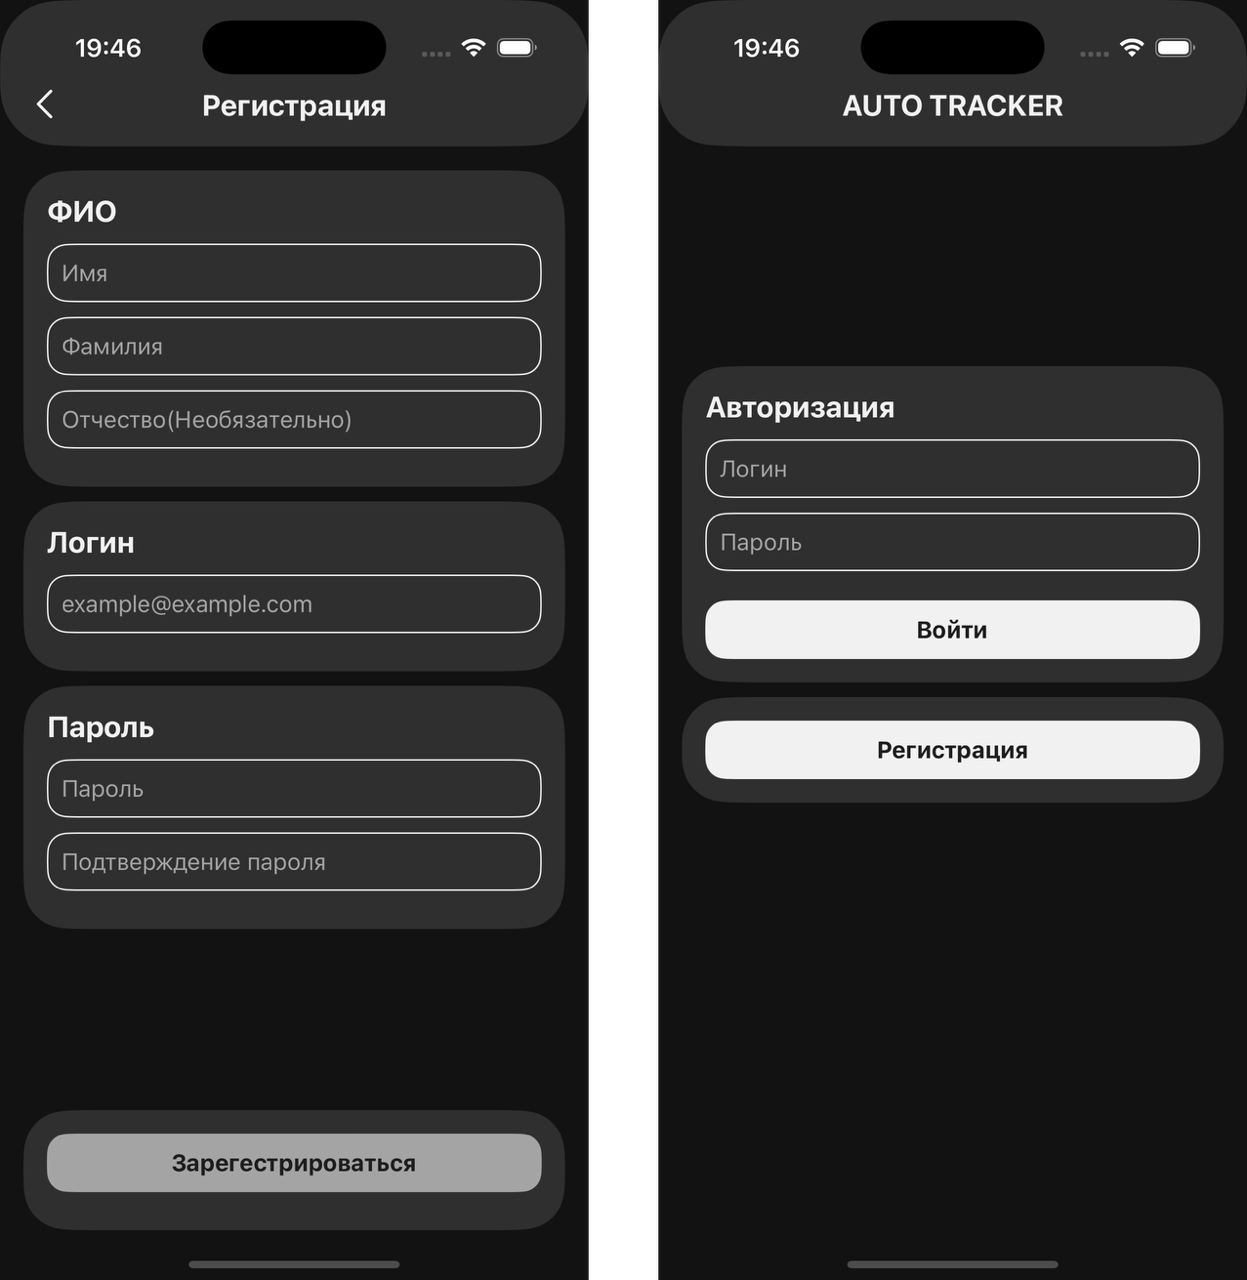
\includegraphics[width=0.6\linewidth]{images/interface/auth.png}
    \caption{Экраны аутентификации}
    \label{fig:int:auth}
\end{figure}
\begin{figure}[H]
    \centering
    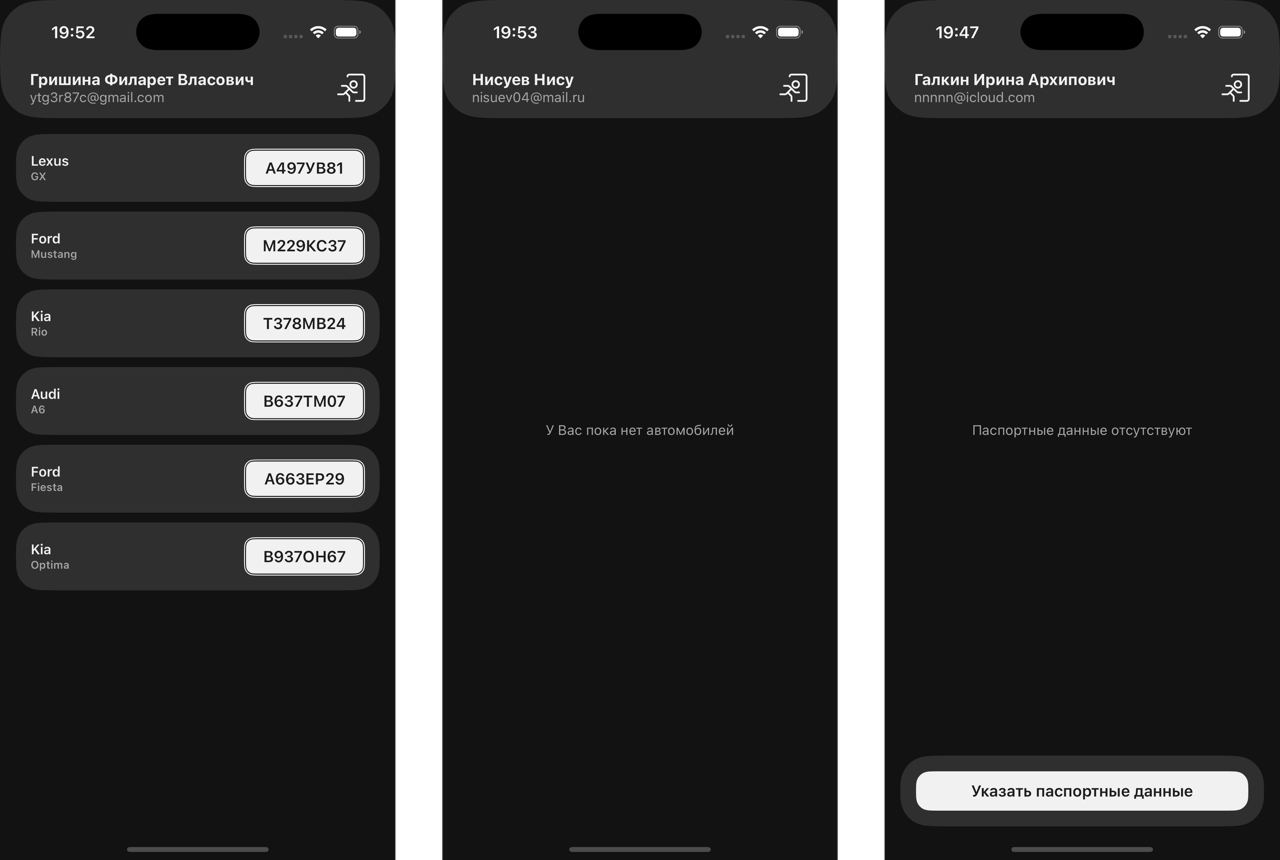
\includegraphics[width=0.8\linewidth]{images/interface/user.png}
    \caption{Экраны пользователя}
    \label{fig:int:user}
\end{figure}
\begin{figure}[H]
    \centering
    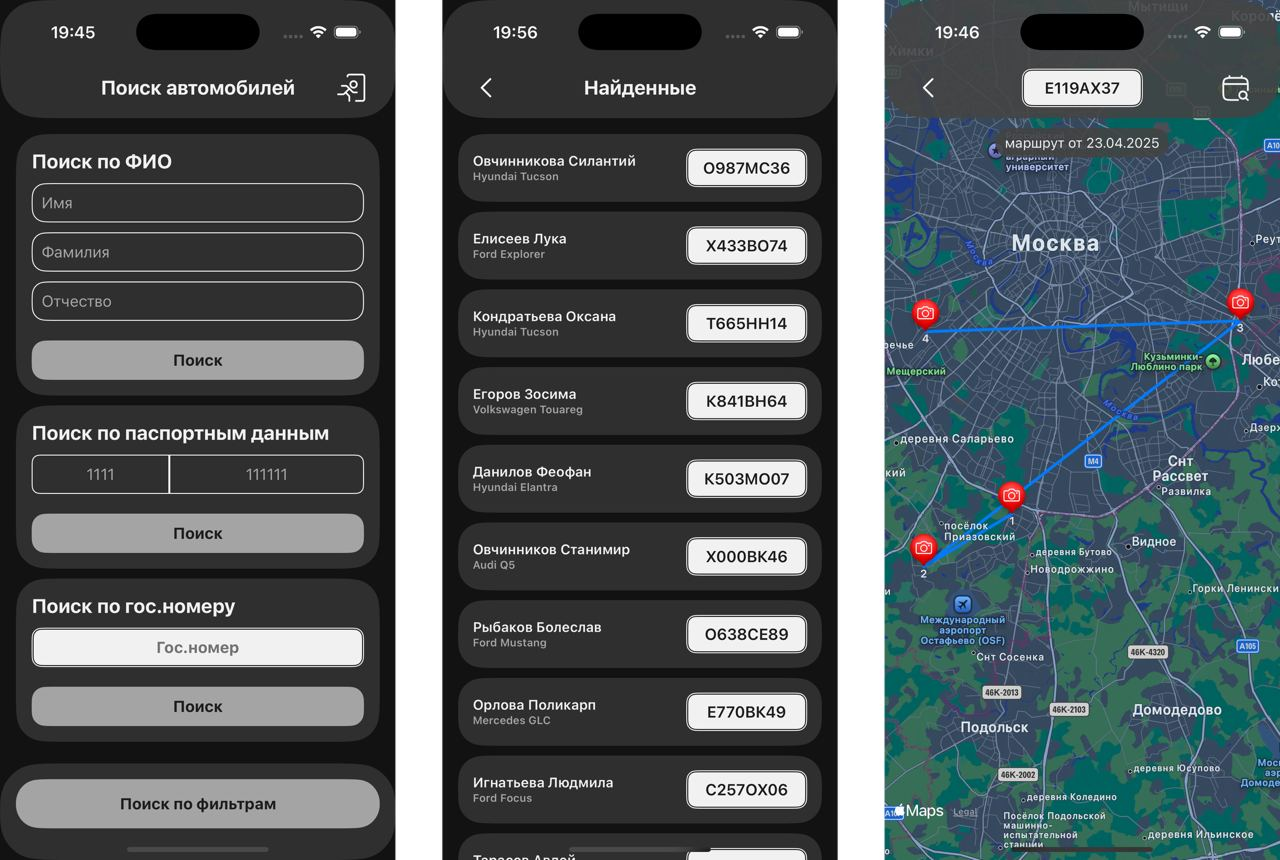
\includegraphics[width=0.8\linewidth]{images/interface/operator.png}
    \caption{Экраны пользователя}
    \label{fig:int:operator}
\end{figure}
\begin{figure}[H]
    \centering
    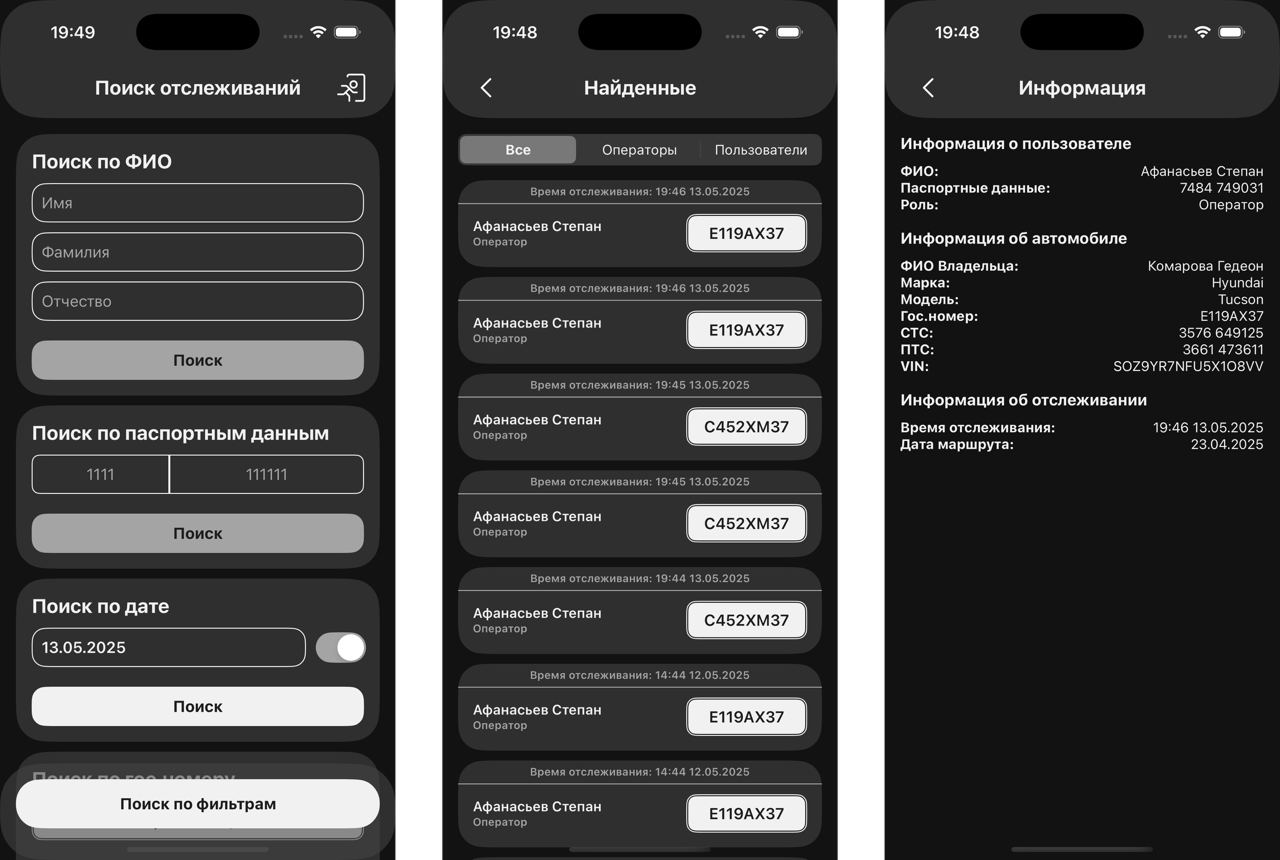
\includegraphics[width=0.8\linewidth]{images/interface/audit.png}
    \caption{Экраны пользователя}
    \label{fig:int:audit}
\end{figure}

Для взаимодействие клиентского приложения с базой данных был разработан API. На рисунке~\ref{fig:int:swagger} представлен Swagger реализованной API.

\begin{figure}[H]
    \centering
    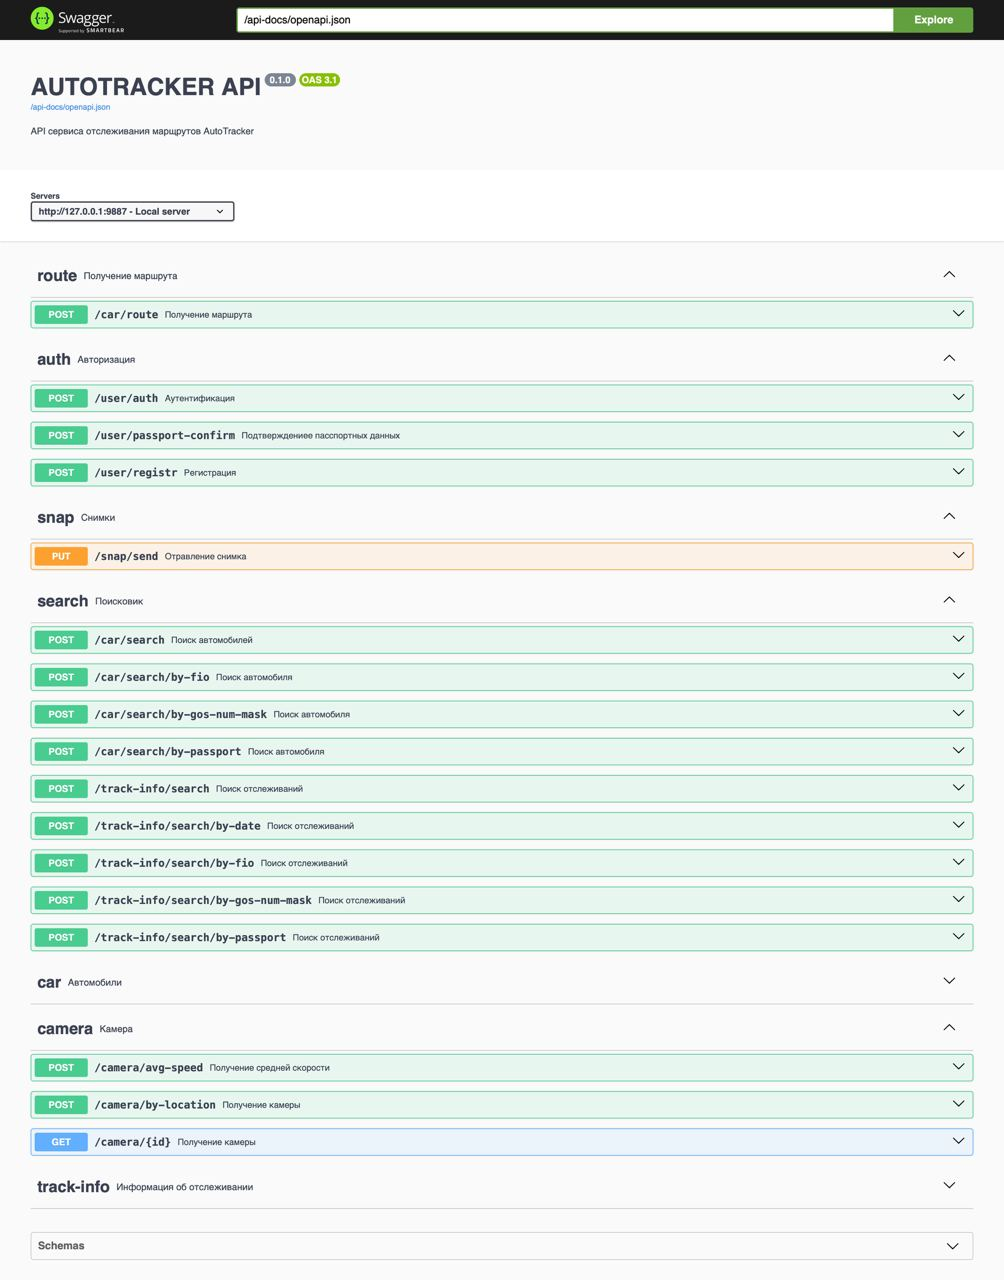
\includegraphics[width=0.8\linewidth]{images/interface/swagger.png}
    \caption{Демонстрация Swagger}
    \label{fig:int:swagger}
\end{figure}

\paragraph*{ВЫВОД} ${}$ \\

В данном разделе были выбраны средства реализации. Представлена реализация сущностей, ролевой модели и ограничений целостности в созданной базе данных. Также рассмотрена реализация хранимой процедуры и проведено ее тестирование. Дополнительно представлен пользовательский интерфейс программного обеспечения.
